\documentclass[tikz,border=3pt]{standalone}
\usepackage[utf8]{inputenc}
\usepackage[T1]{fontenc}
\usepackage{libertinus}
\usepackage{amsmath,amssymb}
\usetikzlibrary{arrows.meta,calc,patterns,decorations.pathmorphing,decorations.markings,decorations.pathreplacing,bending}
\definecolor{UGblue}{RGB}{0,51,102}
\newcommand{\dbar}{\mathchar'26\mkern-12mu d}
\tikzset{
  >=Stealth,
  every node/.style={font=\small},
  caja/.style={draw,line width=0.9pt},
  pared/.style={draw,line width=1.6pt},
  ejes/.style={->,line width=0.8pt},
  adia/.style={draw,pattern=north east lines,pattern color=black!70,line width=0.5pt},
  gas/.style={fill=UGblue!8},
  punto/.style={fill,circle,inner sep=1.3pt},
  onda/.style={decorate,decoration={snake,amplitude=1.1pt,segment length=5pt,post length=3pt,pre length=0pt}},
}
\begin{document}
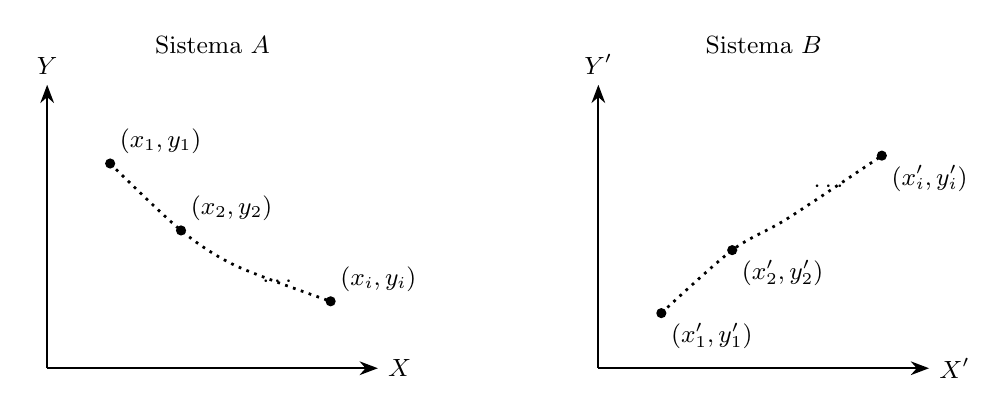
\begin{tikzpicture}
  % sistema A
  \draw[ejes] (0,0) -- (4.2,0) node[right] {$X$};
  \draw[ejes] (0,0) -- (0,3.6) node[above] {$Y$};
  \node at (2.1,4.1) {Sistema $A$};
  \coordinate (a1) at (0.8,2.6); \coordinate (a2) at (1.7,1.75); \coordinate (a3) at (2.4,1.3); \coordinate (a4) at (3.6,0.85);
  \draw[dotted,line width=1pt] plot[smooth] coordinates {(a1) (a2) (a3) (a4)};
  \foreach \p/\t in {a1/{(x_1,y_1)},a2/{(x_2,y_2)},a4/{(x_i,y_i)}} {\node[punto] at (\p) {}; }
  \node[above right] at (a1) {$(x_1,y_1)$};
  \node[above right] at (a2) {$(x_2,y_2)$};
  \node[above right] at (a4) {$(x_i,y_i)$};
  \node at (2.95,1.1) {$\cdots$};
  % sistema B
  \begin{scope}[xshift=7cm]
  \draw[ejes] (0,0) -- (4.2,0) node[right] {$X'$};
  \draw[ejes] (0,0) -- (0,3.6) node[above] {$Y'$};
  \node at (2.1,4.1) {Sistema $B$};
  \coordinate (b1) at (0.8,0.7); \coordinate (b2) at (1.7,1.5); \coordinate (b3) at (2.4,1.9); \coordinate (b4) at (3.6,2.7);
  \draw[dotted,line width=1pt] plot[smooth] coordinates {(b1) (b2) (b3) (b4)};
  \node[punto] at (b1) {}; \node[punto] at (b2) {}; \node[punto] at (b4) {};
  \node[below right] at (b1) {$(x_1',y_1')$};
  \node[below right] at (b2) {$(x_2',y_2')$};
  \node[below right] at (b4) {$(x_i',y_i')$};
  \node at (2.95,2.3) {$\cdots$};
  \end{scope}
\end{tikzpicture}
\end{document}
